\documentclass[a4paper,11pt]{article}
\pdfoutput=1 % if your are submitting a pdflatex (i.e. if you have
             % images in pdf, png or jpg format)

\usepackage{jheppub} % for details on the use of the package, please
                     % see the JHEP-author-manual


\usepackage{hyperref}

\usepackage{amssymb,amsmath,amsfonts}
\usepackage{epsfig}
\usepackage{array}
%\usepackage{verbatim}

\usepackage{tikz}

\usetikzlibrary{calc,through,backgrounds,patterns,decorations.pathmorphing,decorations.markings,%
		trees,positioning,arrows,chains,shapes.geometric,%
    decorations.pathreplacing,shapes}

\usepackage{pgfplots}
%\usepgfplotslibrary{patchplots,fillbetween}

\usepgfplotslibrary{fillbetween}    
\pgfplotsset{compat=1.10}
%\usepackage[dvipsnames]{xcolor}


\usepackage{amsmath}
\usepackage{multirow}
\usepackage{array}
\usepackage{bm}

\newcommand{\vect}[1]{\boldsymbol{\mathbf{#1}}}

\newcommand{\CA}{\mathcal{A}}
\newcommand{\CB}{\mathcal{B}}
\newcommand{\CC}{\mathcal{C}}
\newcommand{\CD}{\mathcal{D}}
%\newcommand{\CE}{\mathcal{E}}
\newcommand{\CF}{\mathcal{F}}
\def\CJ{\mathcal{J}}
\newcommand{\CG}{\mathcal{G}}
\newcommand{\CL}{\mathcal{L}}
\newcommand{\CO}{\mathcal{O}}
\newcommand{\CN}{\mathcal{N}}
\newcommand{\CI}{\mathcal{I}}
\newcommand{\CT}{\mathcal{T}}
\newcommand{\CS}{\mathcal{S}}
\newcommand{\CM}{\mathcal{M}}
\newcommand{\CQ}{\mathcal{Q}}
\newcommand{\CE}{\mathcal{E}}
\newcommand{\CZ}{\mathcal{Z}}

\newcommand{\Z}{\mathbb{Z}}
\newcommand{\C}{\mathbb{C}}
\newcommand{\R}{\mathbb{R}}

\newcommand{\gym}{g_{\rm YM}}

\newcommand{\eps}{\epsilon}
\newcommand{\grad}{\vec{\nabla}}
\newcommand{\el}{\kappa}

\newcommand{\ads}{\mbox{AdS}}

\newcommand{\nn}{\nonumber}
\newcommand{\lspa}{\ \ ,\ \ \ \ }
\newcommand{\spa}{\ , \ \ }

\newcommand{\ds}{\displaystyle}

\newcommand{\tr}{\mathop{{\rm Tr}}}
\DeclareMathOperator{\sgn}{sgn} \DeclareMathOperator{\diag}{diag}

\newcommand{\vecto}[2]{\left( \begin{array}{c} #1 \\ #2 \end{array}
\right) }
\newcommand{\matrto}[4]{\left( \begin{array}{cc} #1 & #2 \\
#3 & #4 \end{array} \right) }
\newcommand{\vectre}[3]{\left( \begin{array}{c} #1 \\ #2\\ #3 \end{array}
\right) }
\newcommand{\matrtre}[9]{\left( \begin{array}{ccc} #1 & #2 & #3 \\ #4 & #5 & #6 \\ #7 & #8 & #9 \end{array} \right) }


\newcommand{\hB}{{}^* \! B}
\newcommand{\hC}{{}^* \! C}
\newcommand{\hF}{{}^* \! F}
\newcommand{\hJ}{{}^* \! J}

\newtheorem{definition}{Definition}[section]
\newtheorem{proposition}[definition]{Proposition}
\newtheorem{theorem}[definition]{Theorem}
\newtheorem{lemma}[definition]{Lemma}
\newtheorem{corollary}[definition]{Corollary}
\newtheorem{comment}[definition]{Comment}
\newtheorem{example}[definition]{Example}
\newtheorem{conjecture}[definition]{Conjecture}

\newcommand{\proof}{\noindent {\bf Proof:}\ }
\newcommand{\squ}{\noindent $\square$}

\newcommand{\bin}[2]{\Big( \begin{array}{c} #1 \\[-1mm] #2 \end{array}
\Big) }

\def\Tr{\mathrm{Tr}}

%---------------------------------------------------------
\numberwithin{equation}{section}
%---------------------------------------------------

\begin{document} 

\section{intro}
\subsection{some formula}
\begin{figure}[h!]
\centerline{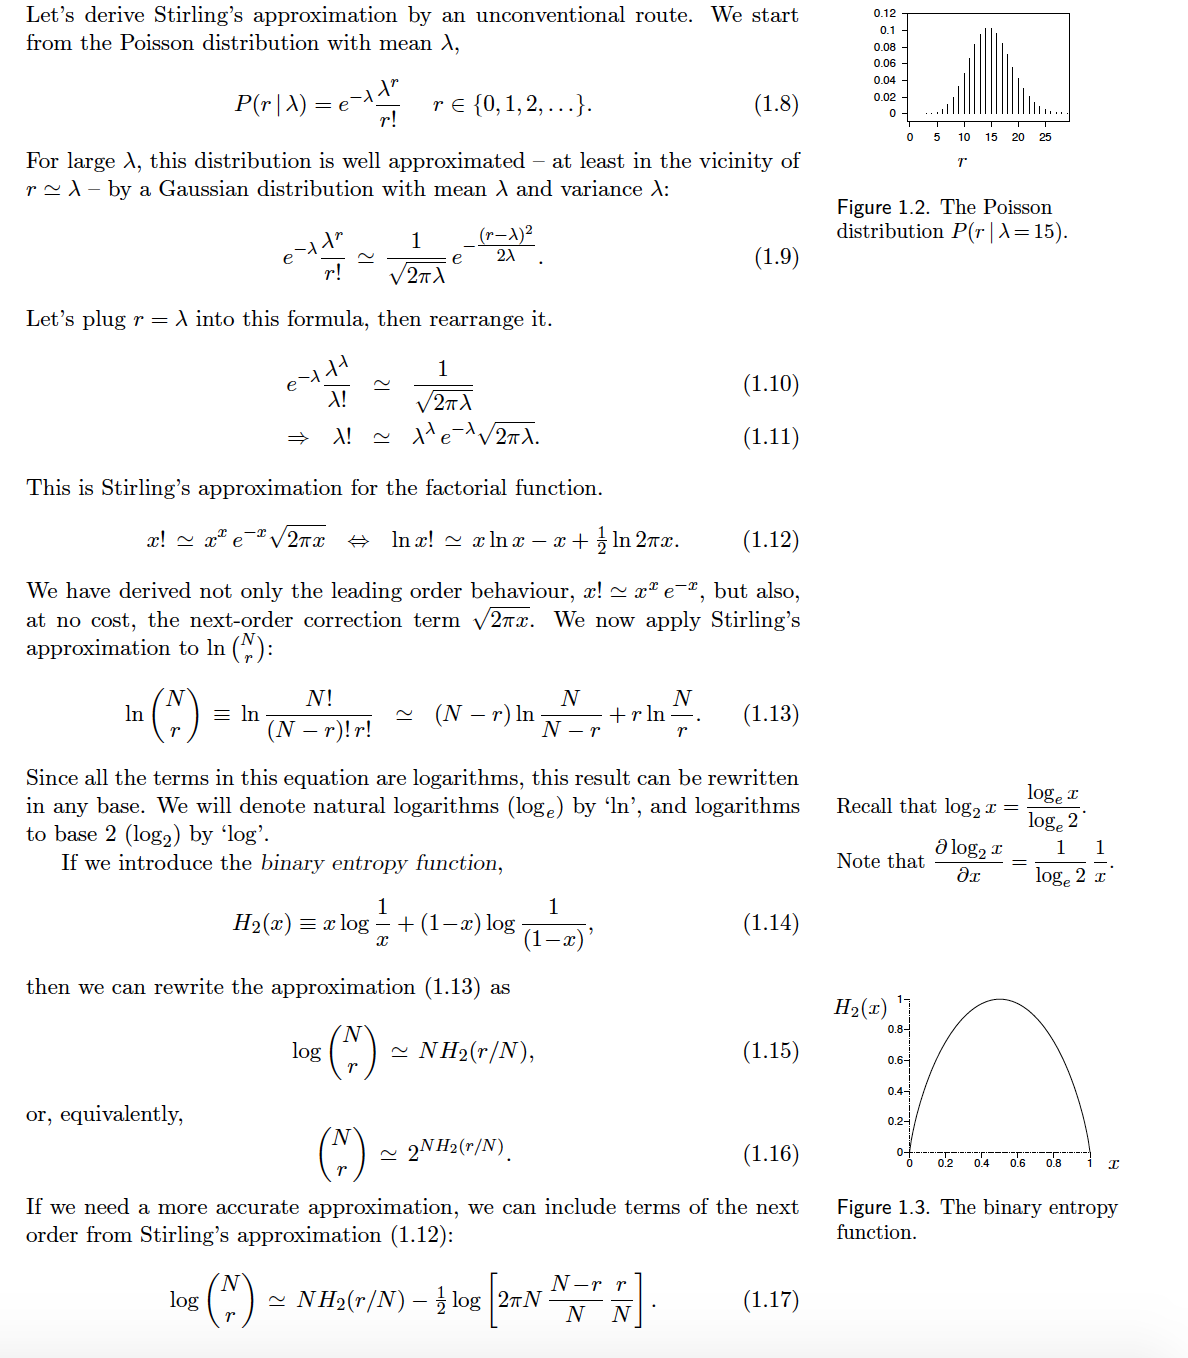
\includegraphics[scale=0.6]{probability_formulae.png}}
\caption{Some formula}
\end{figure}

\subsection{assumptions in inference}

First, once assumptions are made, the inferences are objective and unique,
reproducible with complete agreement by anyone who has the same information
and makes the same assumptions. For example, given the assumptions
listed above, $\mathcal{H}$, and the data D, everyone will agree about the posterior probability
of the decay length
$$
P(\lambda | D, \mathcal{H})= {P(D|\lambda , \mathcal{H})P(\lambda |  \mathcal{H}) \over P(D|\mathcal{H})}
$$

Second, when the assumptions are explicit, they are easier to criticize, and
easier to modify { indeed, we can quantify the sensitivity of our inferences to
the details of the assumptions.



Third, when we are not sure which of various alternative assumptions is
the most appropriate for a problem, we can treat this question as another
inference task. Thus, given data D, we can compare alternative assumptions
$\mathcal{H}$ using Bayes' theorem

$$
P( \mathcal{H}|D,I)= {P(D| \mathcal{H},I)P(\mathcal{H}|I) \over P(D|I)},
$$
where I denotes the highest assumptions, which we are not questioning.

Fourth, we can take into account our uncertainty regarding such assumptions
when we make subsequent predictions. Rather than choosing one particular
assumption $\mathcal{H}^*$, and working out our predictions about some quantity $t$,
$P(t |D, \mathcal{H},I)$, we obtain predictions that take into account our uncertainty 
about H by using the sum rule
$$
P({\textbf t} | D, I)= \sum_{\mathcal{H}} P({\textbf t}|D, \mathcal{H},I)P( \mathcal{H}|D,I) 
$$

This is another contrast with orthodox statistics, in which it is conventional
to `test' a default model, and then, if the test `accepts the model' at some
`significance level', to use exclusively that model to make predictions.
{\it probability theory reaches parts that ad hoc methods cannot reach.}



Model comparison as inference. Assume we have two hypotheses. In order to perform model comparison, We wish to
know how probable $P(\mathcal{H}_1)$ is given the data. By Bayes' theorem,

$$
P( \mathcal{H}_1|{\textbf s},F)= {P(s|F, \mathcal{H}_1)P(\mathcal{H}_1) \over P({\textbf s}|F)},
$$
and 
$$ 
P( \mathcal{H}_0|{\textbf s},F)= {P({\textbf s}|F, \mathcal{H}_0)P(\mathcal{H}_0) \over P({\textbf s}|F)}
$$

The normalizing constant in both cases is the total probability of geting the observed data. and 
$$
P(s|F)=P({\textbf s}|F, \mathcal{H}_1)P(\mathcal{H}_1) +P({\textbf s}|F, \mathcal{H}_0)P(\mathcal{H}_0)
$$

To evaluate the posterior probabilities of the hypotheses we need to assign
values to the prior probabilities $P(\mathcal{H}_1)$ and $P(\mathcal{H}_0)$; in this case, we might
set these to 1/2 each. And we need to evaluate the data-dependent terms
$P(s|F, \mathcal{H}_1)$ and $P(s|F,\mathcal{H}_0)$. We can give names to these quantities. The
quantity $P(s|F, \mathcal{H}_1)$  is a measure of how much the data favour $ \mathcal{H}_1)$, and we
call it the evidence for model $ \mathcal{H}_1)$. {\it How model comparison works : The evidence for a model is usually the normalizing constant of an earlier Bayesian inference.}

\section{Clustering and Maximum Likelihood}
\subsection{Motivation of clustering}
First, a good clustering has
predictive power. Second, clusters can be a useful aid to communication because they allow
lossy compression. A third reason for making a cluster model is that failures of the cluster
model may highlight interesting objects that deserve special attention. A fourth reason for liking clustering algorithms is that they may serve
as models of learning processes in neural systems.

\subsection{K-means}
The K-means algorithm is an algorithm for putting N data points in an M-dimensional space into K clusters. Each cluster is parameterized by a vector
${\textbf m}^{(k)}$ called its mean. 

First of all, set K means {${\textbf m}^{(k)}$} to random values. In the assignment step, each data point n is
assigned to the nearest mean. 
$$
\hat k^{(n)} = argmin_k d({\textbf m}^{(k)}, {\textbf x}^{(n)})
$$
An alternative, equivalent representation of this assignment of
points to clusters is given by `responsibilities', which are indicator
variables $r^{(n)}_k$. In the assignment step, we set $r^{(n)}_k$ to one if mean k is the closest mean to datapoint $ {\textbf x}^{(n)}$; otherwise, $r^{(n)}_k$ is zero.
$$
r^{(n)}_k = \{
\begin{array}{cc}
1 ~~~~~~if ~\hat k^{(n)}=k\\
0 ~~~~~~if ~\hat k^{(n)}\ne k\\
\end{array}
$$
In the update step, the means are adjusted to
match the sample means of the data points that they are responsible for. The update step is very similar to how to find the center of the mass in physics. 
$$
{\textbf m}^{(k)}= {\sum_n ~ r^{(n)}_k {\textbf x}^{(n)} \over R^{(k)}}
$$
where $R^{(k)}$ is the total responsibility of mean $k$
$$
R^{(k)}=\sum_n~r^{(n)}_k
$$




\subsection{Exercise 22.5}
$$
P(k_n = 1|x_n, \vect{\theta})= {P(x_n|k_n=1,\vect{\theta})P(k_n=1,\vect{\theta}) \over P(x_n,\vect{\theta})}
$$
$$
= {P(x_n|k_n=1,\vect{\theta})P(k_n=1,\vect{\theta}) \over \sum_{k_n}  P(x_n|k_n=1,\vect{\theta})P(k_n=1,\vect{\theta}) +P(x_n|k_n=2,\vect{\theta})P(k_n=2,\vect{\theta}) }
$$
where $\vect{\theta}=(\mu_k, ~\sigma_k)$. 
$$
P(k_n=1,\vect{\theta}) \equiv p_1,~~P(k_n=2,\vect{\theta}) \equiv p_2
$$

Then, 
$$
P(k_n=1|x_n,\vect{\theta})= {p_1 \over p_1+p_2 \exp[-(w_1x_n+w0)]}
$$
$$
P(k_n=2|x_n,\vect{\theta})= {p_2 \over p_2+p_1 \exp[-(w_1x_n+w0)]}
$$
where $w_1=2(\mu_1-\mu_2)$, $w_0=-(\mu_1-\mu_2)(\mu_1+\mu_2)$

$$
P(k_n=k|x_n,\vect{\theta}) \equiv p_{k|n}
$$

By assumption, the prior probability $p_1=p_2=1/2$ then, (22.17) of the book is satisfied. 
$$
L\equiv \log \Pi_n P(x_n|\{\mu_k\},~\sigma)
$$
then trivially, 
$$
{\partial \over \partial{\mu_k}}L = \sum_n  {p_{k|n} (x_n-\mu_k)\over \sigma^2}
$$
$$
{\partial^2 \over \partial{\mu_k}^2}L = -\sum_n  {p_{k|n}  \over \sigma^2}
$$
The new updated $\vect \mu'$ should maximize the likelihood. Then,
$$
{\partial \over \partial{\mu_k'}}L = \sum_n  {p_{k|n} (x_n-\mu_k')\over \sigma^2}=0
$$
$$
\sum_n p_{k|n} ~x_n - \sum_n p_{k|n} ~\mu'_k=\sum_n p_{k|n} ~x_n -  \mu'_k\sum_n p_{k|n}=0
$$
Therefore,
$$
\mu'_k={\sum_n p_{k|n} ~x_n \over \sum_n p_{k|n} }
$$
Note that this equation is exactly the same as the updated means from the responsibilities and data points in soft K-means clustering. $p_{k|n}$ is the responsibility $r^{(k)}_n$.

$$
{{\partial \over \partial{\mu_k}}L \over {\partial^2 \over \partial{\mu_k}^2}L  } = {\sum_n p_{k|n} ~x_n -  \mu_k\sum_n p_{k|n} \over -\sum_n p_{k|n}}= -\mu'_k+\mu_k
$$
Thus, 
$$
\mu'_k=\mu_k-{{\partial \over \partial{\mu_k}}L \over {\partial^2 \over \partial{\mu_k}^2}L  }
$$

\subsection{Exercise 22.15}
$$
N=7
$$
$$
x_n=(-27.02, 3.57, 8.191, 9.898, 9.603, 9.945, 10.056)
$$
$$
{\sum_n x_n\over N}=3.46329
$$
It must not be the correct mean. 

The likelihood is as followings by the description of the problem. 
$$
P(\{x_n\}|\sigma_n,\mu) = ({1 \over 2\pi })^{N/2} \Pi_n{1\over \sigma_n } \exp(-\sum_n {(x_n-\mu)^2 \over 2\sigma^2_n})
$$ 
To find the maximum likelihood,
$$
L \equiv \log P(\{x_n\}|\sigma_n,\mu) = -\sum_n \log~\sigma_n-\sum_n {(x_n -\mu)^2 \over 2\sigma_n^2} =0 
$$
$$
{\partial L \over \partial x_n} = -\sum_n \left({x_n-\mu \over \sigma^2_n}\right)=-\sum_n{x_n \over \sigma_n^2}+\mu\sum_n {1 \over \sigma_n^2}
$$
$$
\mu= {\sum_n{x_n\over \sigma_n^2}\over{1\over \sigma_n^2}}
$$
When $x_n=(-27.02, 3.57)$, the correspondent $\sigma_n$ are so huge, then it contributes very tiny in $\mu$. Then, the mean should be close to mean of $(8.191, 9.898,$ 
$9.603, 9.945, 10.056)$.


\subsection{Exercise 24.3}

The setting is same as the exercise 22.15.

Bayesian for posterior probability of $\sigma_n$ is 
$$
P(\sigma_n|\{x_n\},\mu)= {P(\{x_n\}|\sigma_n,\mu) P(\sigma_n)\over P(\{x_n\}|\mu)}
$$
Given
$$
P(\{x_n\}|\sigma_n,\mu) = ({1 \over 2\pi })^{N/2} \left( \Pi_n{1\over \sigma_n }\right) \exp\left(-\sum_n {(x_n-\mu)^2 \over 2\sigma^2_n}\right)
$$ 
and
$$
P(\sigma_n)=({1\over \Gamma(c)~s^c})^N\Pi_n~(\sigma_n)^{c-1}~\exp({\sum_n \sigma_n \over s})\footnote{not sure if it is right.}
$$
where $(s,~c)=(10,0.1)$.

and the normalizing constant is
$$
P(\{x_n\}|\mu)=\int^{\infty}_0~\Pi_n~d\sigma_n ~P(\{x_n\}|\sigma_n,\mu) P(\sigma_n)
$$


\begin{figure}
\centerline{
\begin{tabular}{cc}
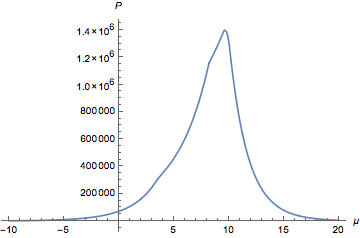
\includegraphics[width=.5\textwidth]{7scientistplot.png} &
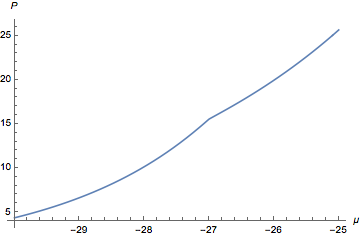
\includegraphics[width=.5\textwidth]{7scientistplot2.png}
\end{tabular}}
\caption[The plot of exercise 24.3]{\label{7scientist} \small The distribution functions are not normalized yet. However, this plot already shows the maximum likelihood should be around $\mu=10$. The small bumps around $x_n=(-27,~3.6,~8)$ are also seen in the graph. }
\end{figure}


The posterior probability of $\mu$ is 
$$
P(\mu|x_n)={P(\{x_n\}|\mu)P(\mu)\over P(\{x_n\})}
$$
and the prior is determined by some assumption. 
$P(\mu) = {1 \over \sigma_{\mu}}=const.$, then the normalizing constant is  
$$
P(\{x_n\})=\int^{\infty}_{-\infty} ~d\mu ~P(\{x_n\}|\mu)  {1 \over \sigma_{\mu}}
$$




\section{Monte Carlo }

\subsection{Laplace approximation}
\subsubsection{Exercise 27.1}
$r$ is a positive integer, and posterior over lambda
$$
P(\lambda|r)= {P(r|\lambda) P(\lambda)\over P(r)}
$$

$$
P(r|\lambda)=\exp(\lambda){\lambda^r \over r!}
$$
By assumption
$$
P(\lambda)={1\over \lambda}
$$
Then, the normalizing constant is 
$$
P(r)=\int^{\infty}_0~d\lambda~ \exp(\lambda){\lambda^r \over r!}{1\over \lambda}= {\Gamma(r) \over r!} = {1\over r}
$$
We need to find the $lambda$ for maximum likelihood. By differentiate the posterior probability distribution function with respect to $\lambda$, 
it has a maximum at $\lambda = \lambda_0=r-1$, and 
$$
P(\lambda=\lambda_0=r-1|r)={(r-1)^{(r-1)}\exp(r-1)\over (r-1)!}
$$
$$
c=-{\partial^2 \over \partial \lambda^2}\log~P(\lambda|r)|_{\lambda=\lambda_0=r-1}={1-r \over \lambda^2}|_{\lambda=\lambda_0=r-1}={1\over r-1}
$$ 

Then, the Laplace approximation is 
$$
G(\lambda|r)= P(\lambda=\lambda_0=r-1|r)\exp\left(-{c\over 2}{(\lambda-\lambda_0)^2}\right)
$$


\begin{figure}
\centerline{
\begin{tabular}{cc}
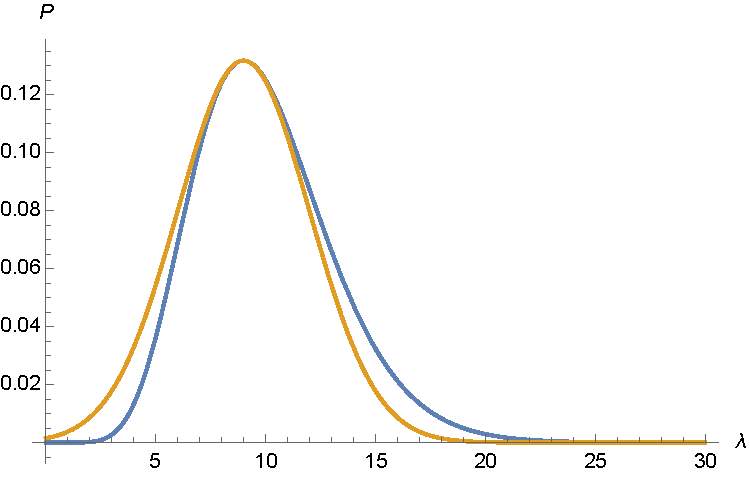
\includegraphics[width=.5\textwidth]{laplace.pdf} &
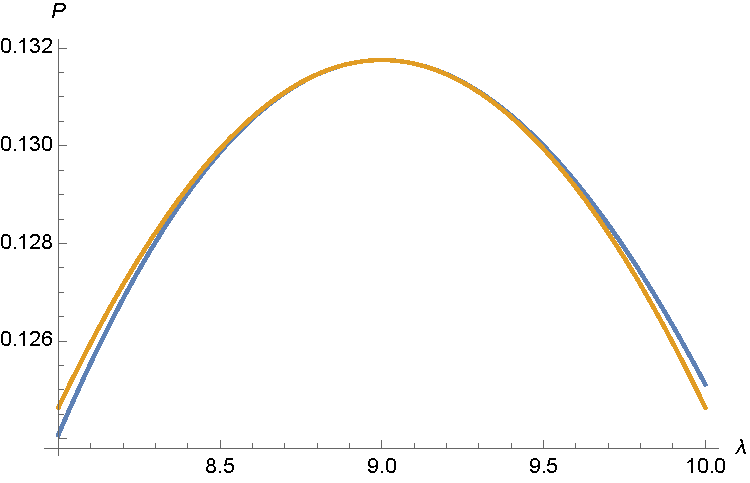
\includegraphics[width=.5\textwidth]{laplace2.pdf}
\end{tabular}}
\caption[The plot of exercise 27.1]{\label{laplace} \small $r=10$ is set. The blue plot is Poisson distribution and the orange one is the Laplace approximation. 
%%% Look into the plot around the maximum. Very well matched around the tip. The maximum is at $r=9$.The blue plot is Poisson distribution and the orange one is the Laplace approximation. Poisson distribution is not symmetric about the axis of $r=9$. Laplace approximation is symmetric and has same maximum and variance. 
%%%
}
\end{figure}

\subsubsection{Exercise 27.3}

Bayesian for posterior of $\omega_0, \omega_1$. $y(x_n)$ is the mean of $t_n$ data points. 

$$
P(\{\omega_i\}|t_n,x_n, \sigma_{\nu})= { P(t_n|\{\omega_i\},x_n,\sigma_{\nu})P(\omega_0)P(\omega_1)\over P(t_n|x_n\sigma_{\nu})}\footnote{not sure if it is correct yet. I am still confused at Bayesian theory.}
$$
$P(t_n|\{\omega_i\},\sigma_{\nu})$, $P(\omega_0)$, $P(\omega_1)$ are all Gaussian distributed. Prior $P(\omega_0)$, $P(\omega_1)$ are assumed to be Gaussian. 

$$
P(t_n|\sigma_{\nu})= \int^{\infty}_{-\infty} d\omega_0 \int^{\infty}_{-\infty} d\omega_1~ P(t_n|\{\omega_i\},\sigma_{\nu})P(\omega_0)P(\omega_1)
$$

$$
P(\{t_n\}|\{\omega_i\},x_n,\sigma) = ({1 \over 2\pi \sigma^2_{\nu}})^{N/2}  \exp\left(-\sum_n {(t_n-y(x_n))^2 \over 2\sigma^2}\right)
$$
$$
y(x_n)=\omega_0 + \omega_1 x_n
$$
$$
P(\omega_i)=  ({1 \over 2\pi \sigma^2})^{1/2}  \exp\left(-{\omega_i^2 \over 2\sigma_i^2}\right)
$$
Because the mean of $\omega_i$ should be zero obviously, and the variances of $\omega_0$ and $\omega_1$, i.e. $\sigma_1$, $\sigma_2$ could be same without loss of generality. The variance of $t_n$ would have a very broad range of values dependent on $x_n$. I assumed $\sigma_i^2 = \sigma/3$ at Figure \ref{BayesianRegression}.  

To use Laplace approximation, find $\{\omega_i\}$ satisfy ${\partial \over \partial \omega_i}\log P(\{\omega_i\}|t_n,x_n, \sigma)$. \footnote{Do you have any better suggestion?}

\begin{equation}\label{blr}
\log P(\{\omega_i\}|t_n,x_n, \sigma) = -\left(\sum_n {(t_n-\omega_0 - \omega_1 x_n)^2 \over 2\sigma^2}\right)-{\omega_0^2 \over 2\sigma_0^2}-{\omega_1^2 \over 2\sigma_1^2}
\end{equation}

Some reader might notice that $-\sum_n {(t_n-\omega_0 - \omega_1 x_n)^2 \over 2\sigma^2}$ term is minimized for the linear regression. We have two extra terms from the priors. It is {\it Bayesian linear regression}.  

By the way, $\omega_0^*$ and $\omega_1^*$ satisfy Eq. \ref{blr} is quite complicated. I tried to find the simplified form, but can't. I would just keep symbolic expressions of $\omega_0^*$, $\omega_1^*$. 


Using the Eq. (27.6) of the book,
$$
\vect A={1\over \sigma^2}\left(
\begin{array}{ccc}
N+1 & -\sum_n x_n  \\
  -\sum_n x_n  & (\sum_n x_n)^2 + 1 \\
\end{array}
\right)
$$


Then, the Laplace approximation is 

$$
G(\{\omega_i\}|t_n)= P(\{\omega_i^*\}|t_n,x_n, \sigma) exp\left(  -{1 \over 2} (\vect \omega - \vect \omega_0)^T \vect A  (\vect \omega - \vect \omega_0)\right)
$$
where $ \vect \omega  = (\omega_0, \omega_1)$ and $ \vect \omega^*  = (\omega_0^*, \omega_1^*)$


\begin{figure}
\centerline{
\begin{tabular}{cccc}
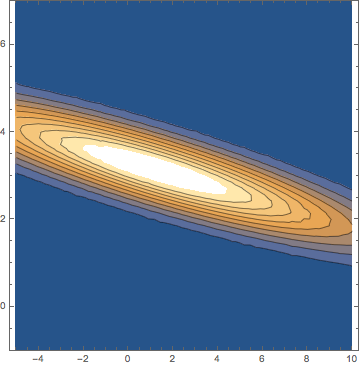
\includegraphics[width=.4\textwidth]{Likelihood.png} &
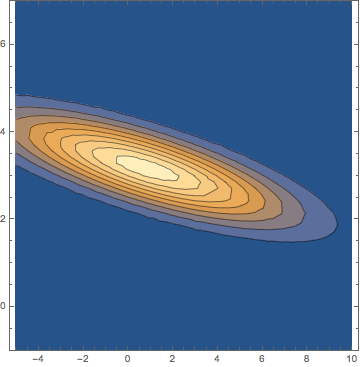
\includegraphics[width=.4\textwidth]{BayesianRegression.png} &
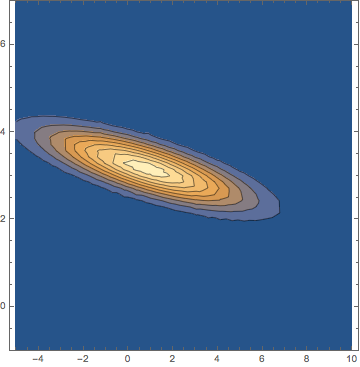
\includegraphics[width=.4\textwidth]{BayesianRegression2.png}&
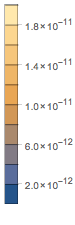
\includegraphics[width=0.1\textwidth]{BayesianRegression3.png}
\end{tabular}}
\caption[The plot of exercise 27.3]{\label{BayesianRegression} \small The likelihood and posterior probability distribution plot and its Laplace approximation. I have put 10 random data points $x_n$ and $t_n ~ 3x_n+2 \pm 2$. The left plot has the maximum likelihood around $(\omega_0, \omega_2) = (1.79794, 3.02217)$, and the central posterior is about $(\omega_0, \omega_2) = (0.812961, 3.16977)$. The discrepancy occurs by the assumed priors. Because the mean of $\omega_i$ should be zero obviously, and the variances of $\omega_0$ and $\omega_1$, i.e. $\sigma_1$, $\sigma_2$ could be same without loss of generality. The variance of $t_n$ would have a very broad range of values dependent on $x_n$. I assumed $\sigma_i^2 = \sigma/3$. It is chosen from base of the mean value of $x_n$. The last one is obtained by Laplace approximation. I did not normalize them.}
\end{figure}


\subsection{Occam's razor}

This section is very well summarized at the figures of the book. Occam's factor is defined in the process of model comparison. The Occam's factor ${\sigma_{\omega|D}\over \sigma_{\omega}}$ is equal to the ratio of the posterior accessible volume of $\mathcal{H}_i$'s parameter space to the prior accessible volume, or the factor by which $\mathcal{H}_i$'s hypothesis space collapses when the data arrive. The factor is smaller as the model is simple. The logarithm of the Occam factor is a measure of the amount of
information we gain about the model's parameters when the data arrive.

{\it Occam factor for several parameters}
If the posterior is well approximated by a Gaussian, then the Occam factor
is obtained from the determinant of the corresponding covariance matrix (cf.
equation (28.8) and Chapter 27):

$$
P(D|\mathcal{H}_i) \sim P(D|\vect w_{MP}, \mathcal{H}_i) \times P(\vect w_{MP}| \mathcal{H}_i) \det (\vect A/2\pi)^{-1/2}
$$ 
$~~~~~~~~~~~$Evidence $\sim$ Best fit likelihood $\times$ Occam factor

where $\vect A = -\Delta \Delta \log P(D|\vect w_{MP}, \mathcal{H}_i)$. Bayesian model comparison is a simple extension of maximum likelihood model selection: the evidence is obtained by multiplying the best-fit likelihood by the Occam factor. To evaluate the Occam factor we need only the Hessian $\vect A$, if the Gaussian
approximation is good. Thus the Bayesian method of model comparison by
evaluating the evidence is no more computationally demanding than the task
of finding for each model the best-fit parameters and their error bars.


\subsubsection{Exercise 28.1}

For given $x= 0.3,0.5,0.7,0.8,0.9$, which hypothesis would be more probable? By intuition, $\mathcal{H}_0$, because the data looks rather uniformly distributed. 

$P(D|\mathcal{H}_0)$ is ${1 \over 2}\times {1 \over 2} \times{1 \over 2} \times{1 \over 2}\times {1 \over 2}  = 0.03125$ since the probability distribution is uniform. 

$P(D|\mathcal{H}_1)$ is a product of ${1 \over 2} (1- 0.4 x)$ for $x= 0.3,0.5,0.7,0.8,0.9$. It is about $0.00689357$. The ratio ${P(D|\mathcal{H}_0) \over P(D|\mathcal{H}_1)} \sim 4.53321$. $P(D|\mathcal{H}_0)$ is 4.5 times more probable. 

\subsubsection{Exercise 28.2}

Look at the data points plot. 

\begin{figure}[h!]
\centerline{
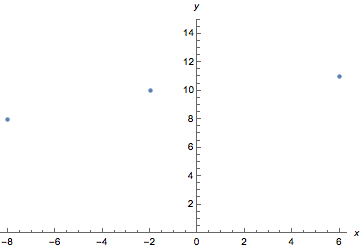
\includegraphics[width=.7\textwidth]{datapointsExercise28-2.png}}
 \caption[The plot of exercise 28.2-1]{\label{Exercise28-2-1} \small }
\end{figure}

The best fit would be almost flat but the slope is not zero, and the y-intersection would be around 10. Which hypothesis is more probable by your intuition? 


The given data points,D= (x, t)= \{(-8, 8), (-2, 10), (6, 11)\};
The evidence is  

{\small 
$$
P(D|\sigma_{\nu}, \sigma_{\omega_0},\sigma_{\omega_1},\mathcal{H}_i) = \int^{\infty}_{-\infty} d\omega_0 \int^{\infty}_{-\infty} d\omega_1 P(D|\omega_0, \omega_1,\sigma_{\nu}, \mathcal{H}_i) P(\omega_0| \sigma_{\omega_0},\sigma_{\omega_1},\mathcal{H}_i)P(\omega_1| \sigma_{\omega_0},\sigma_{\omega_1},\mathcal{H}_i)
$$ }

For $\mathcal{H}_2$,
{\tiny
$$
P(D|\sigma_{\nu}, \sigma_{\omega_0},\sigma_{\omega_1},\mathcal{H}_2) = \int^{\infty}_{-\infty} d\omega_0 \int^{\infty}_{-\infty} d\omega_1 
{1\over \sqrt{2\pi }\sigma_{\nu}} 
\exp\left(-{(\omega_0+\omega_1 x - t)^2\over 2\sigma^2_{\nu}}\right){1\over \sqrt{2\pi }\sigma_{\omega_0}} 
\exp\left(-{(\omega_0-\mu_{\omega_0})^2\over 2\sigma^2_{{\omega_0}}}\right){1\over \sqrt{2\pi }\sigma_{\omega_1}} 
\exp\left(-{(\omega_1-\mu_{\omega_1})^2\over 2\sigma^2_{{\omega_1}}}\right)
$$ }

Then, the evidence for $\mathcal{H}_2$ with respect to 3 data points are about $0.0302393, ~0.0000391484, ~0.0131697$ for each. The total evidence is about $1.55905 \times 10^{-8}$.



For $\mathcal{H}_1$, $\omega_1 =0$ is fixed, so we do not have related term. 
{\small $$
P(D|\sigma_{\nu}, \sigma_{\omega_0},\sigma_{\omega_1},\mathcal{H}_1) = \int^{\infty}_{-\infty} d\omega_0 \int^{\infty}_{-\infty} d\omega_1 
{1\over \sqrt{2\pi }\sigma_{\nu}} 
\exp\left(-{(\omega_0+\omega_1 x - t)^2\over 2\sigma^2_{\nu}}\right){1\over \sqrt{2\pi }\sigma_{\omega_0}} 
\exp\left(-{(\omega_0-\mu_{\omega_0})^2\over 2\sigma^2_{{\omega_0}}}\right)
$$ }

The evidence for $\mathcal{H}_1$ with respect to 3 data points are about $3.17456 \times 10^{-8},~3.91772 \times 10^{-12},~2.05583 \times 10^{-14}$ for each. The total evidence is about $2.55684 \times 10^{-33}$.

Therefore, the horizontal line has much smaller evidence, and it agrees with the intuition. 



\end{document}






